Dentre as CNNs mais profundas, a primeira a ser considerada para estar presente neste trabalho foi a VGG-16. Para esta arquitetura, foi feita a escolha de hiperparâmetros de maneira arbitrária. Primeiramente, preferiu-se trabalhar com a função de ativação ReLU, porém, após a percepção da não convergência dos modelos ajustados com esta função, devido ao \emph{Dying ReLU problem}. A demonstração de \emph{loss} e acurácia durante o treinamento deste primeiro modelo adotado pode ser visualizada na Figura \ref{fig:vgg-dying-relu}.


\begin{figure}[H]
\centering
\caption{Histórico de \emph{loss} e acurácia durante o treinamento de um modelo degenerado obtido com a arquitetura VGG-16.}
\label{fig:vgg-dying-relu}
\subfloat[\emph{Loss} durante treinamento da rede VGG-16 degenerada.\label{subfig:vgg-b-loss}]{%
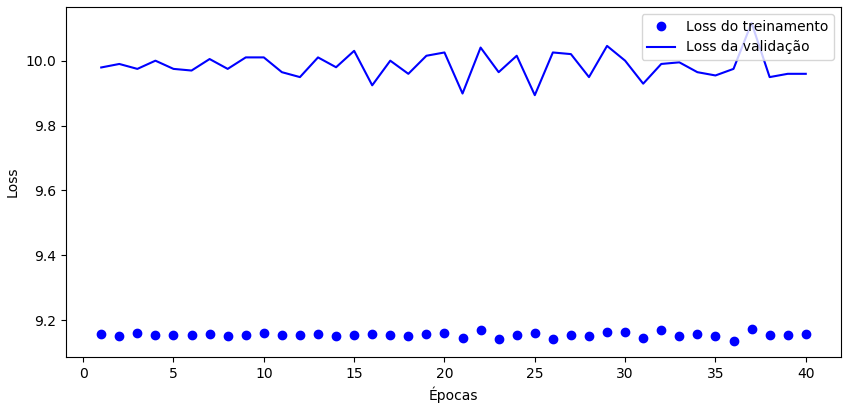
\includegraphics[width=0.47\textwidth]{imgs/vgg-dying-relu-loss}
}
\hfill
\subfloat[Acurácia durante treinamento da rede VGG-16 degenerada.\label{subfig:vgg-b-acc}]{%
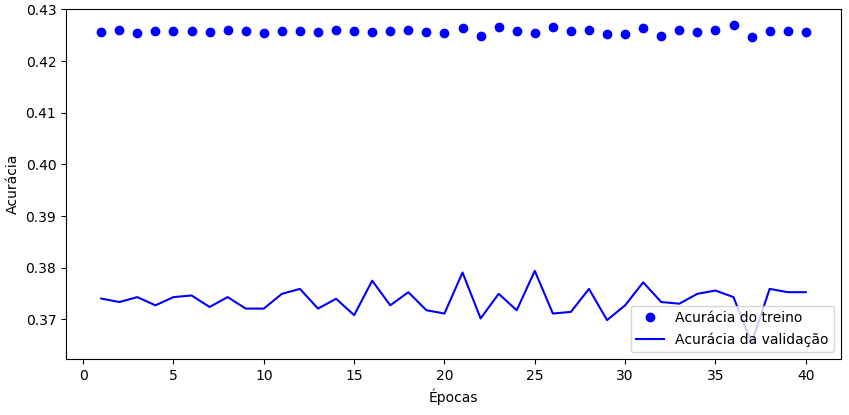
\includegraphics[width=0.47\textwidth]{imgs/vgg-dying-relu-acc}
}
\end{figure}

Após estes resultados, consequentemente, optou-se por utilizar a função de ativação ELU para a obtenção de apenas um modelo para a abordagem B. A escolha do desenvolvimento de uma única rede VGG se deu devido ao longo tempo de treinamento de modelos para este tipo de arquitetura. 

Com a intenção de obter bons resultados, durante o treinamento do modelo, foi utilizado o método \emph{model checkpoint} do Keras, o qual salva os pesos do modelo quando a acurácia do conjunto de validação, neste caso, é a melhor encontrada durante todo o processo de treinamento. Utilizando o último modelo salvo na etapa de testes, tem-se as métricas e os hiperparâmetros expostos na Tabela \ref{fig:treinamento-vgg}. A Figura \ref{fig:treinamento-vgg} mostra o histórico de \emph{loss} e acurácia deste único modelo.

\begin{table}[h!]
\centering
\caption{Detalhamento do modelo obtido com a arquitetura VGG-16 para a abordagem B.}
\label{tab:vgg}
\begin{tabular}{cccccc}
\toprule
\textbf{Otimizador} & \textbf{\emph{Patience}}  & \textbf{Função de Ativação} & \textbf{Acurácia} & \textbf{F-Score} & \textbf{EER} \\
\midrule
RMSprop & 10 & ELU & $0.8391$ & $0.8019$ & $16.1096$ \\
\bottomrule
\end{tabular}
\end{table}

\begin{figure}[H]
\centering
\caption{Histórico de \emph{loss} e acurácia durante o treinamento do modelo obtido com a arquitetura VGG-16.}
\label{fig:treinamento-vgg}
\subfloat[\emph{Loss} durante treinamento da rede VGG-16 para a abordagem B.\label{subfig:vgg-b-loss}]{%
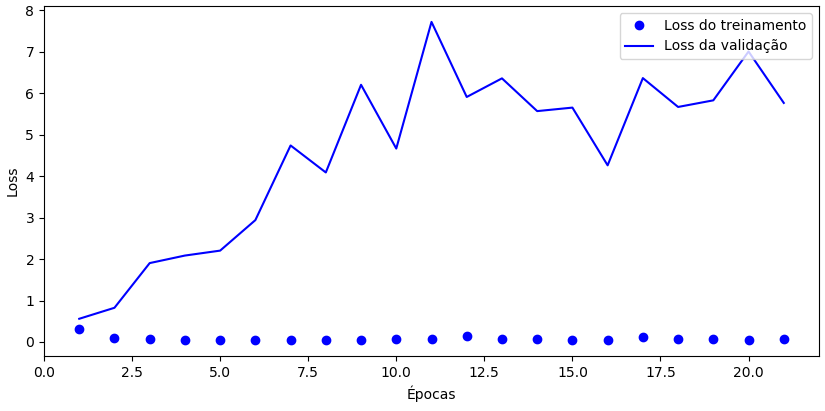
\includegraphics[width=0.47\textwidth]{imgs/vgg-b-loss}
}
\hfill
\subfloat[Acurácia durante treinamento da rede VGG-16 para a abordagem B.\label{subfig:vgg-b-acc}]{%
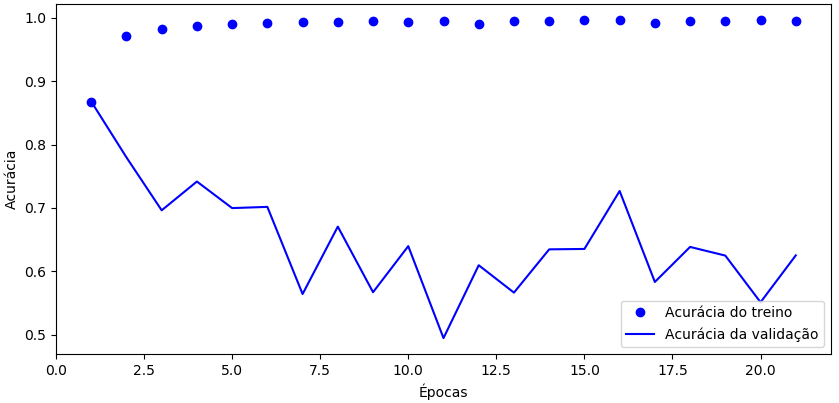
\includegraphics[width=0.47\textwidth]{imgs/vgg-b-acc}
}
\end{figure}

A matriz de confusão deste modelo, disposta na Figura \ref{fig:matrizes-vgg}, mostra mais uma vez uma diagonal principal bastante densa, enquanto que a diagonal secundária está bem distribuída entre previsões forjadas e autênticas. Estes valores estão refletidos nas métricas de desempenho apresentadas na Tabela \ref{tab:vgg}.

\begin{figure}[h]
    \centering
    \caption{Matriz de confusão do modelo obtido com a arquitetura VGG-16.}\label{fig:matrizes-vgg}
    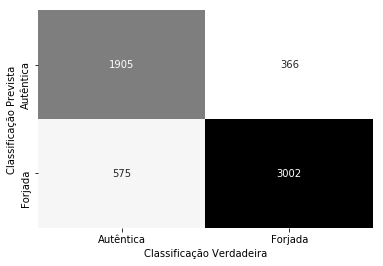
\includegraphics[width=0.6\textwidth]{imgs/matriz-vgg}
\end{figure}

Em suma, este modelo pôde mostrar que esta arquitetura pode ser útil para lidar com a tarefa de aprendizado proposta. Contudo, cabe observar que a utilização desta CNN pode ser demais para trabalhar com imagens com poucos padrões, como é o caso.